
\begin{minipage}[t][0.6\textheight][t]{\textwidth}
\begin{columns}
\column{0.5\textwidth}
\begin{overlayarea}{\textwidth}{\textheight}
\justify
\only<1>{\myheading{Unsupervised Pre-Training}}
\only<1>{Hinton and  Salakhutdinov described an effective way of initializing the weights that allows deep autoencoder networks to learn a low-dimensional representation of data. \cite{Salakhutdinov:2012:ELP:2330716.2330717}}
\end{overlayarea}
\column{0.5\textwidth}
\begin{overlayarea}{\textwidth}{\textheight}
\begin{figure}
\centering
\only<1>{\includegraphics[scale=0.7]{"images/Renewed_Interest/2006_1"}}
%\only<2>{\includegraphics[scale=0.5]{"Renewed_Interest/2009"}}
%\only<3>{\includegraphics[scale=0.5]{"Renewed_Interest/2010_1"}}
%\only<4>{\includegraphics[scale=0.5]{"Renewed_Interest/2010"}}
%\only<5>{\includegraphics[scale=0.5]{"Renewed_Interest/2011"}}
%\only<6>{\includegraphics[scale=0.5]{"Renewed_Interest/2012_1"}}
%\only<7>{\includegraphics[scale=0.5]{"Renewed_Interest/2012_1"}}
\end{figure}
\end{overlayarea}
\end{columns}
\end{minipage}
\begin{minipage}[t][0.4\textheight][t]{\textwidth}
\begin{columns}
\column{0.1\textwidth}
\column{0.9\textwidth}
\begin{overlayarea}{\textwidth}{\textheight}
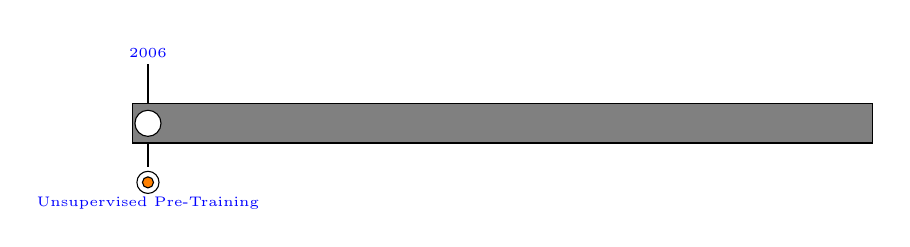
\begin{tikzpicture}[datemarker/.style={circle, draw=black,fill=white},textlabel/.style={anchor=center,text height=1.7ex,text depth=.25ex}] 
\tikzset{every node/.style={font=\tiny, color=blue}}\draw[fill=gray](-0.2,0) rectangle (9.2,0.5) node[white, below]{}; 
\onslide<1>{\node at (0.0, 0.25) [datemarker] {};}
\onslide<1>{\draw [line width=1pt] (0.0, 0.5) to (0.0, 1.0);} 
\onslide<1>{\draw (0.0, 1.2) node [textlabel] {2006 };}
\onslide<1>{\draw [fill=orange](0.0, -0.5) circle (2pt){};}
\onslide<1>{\draw (0.0, -0.5) circle (4pt){};}
\onslide<1>{\draw [line width=1pt] (0.0, 0) to (0.0, -0.3);}
\onslide<1>{\draw (0.0,-0.7) node [textlabel] {Unsupervised Pre-Training};}
\end{tikzpicture}
\end{overlayarea}
\end{columns}
\end{minipage}